
\documentclass[10pt,openany,a4paper]{article}
\usepackage{tikz, pgfplots, tkz-euclide,calc}
\usetikzlibrary{patterns,shapes.arrows,calc}
\usepackage{fancyhdr}
\usepackage{enumerate,enumitem}
\usepackage{cancel}
\usepackage{varwidth}

% TAMBAHKAN PACKAGE SENDIRI KALAU KURANG

\usepackage{geometry}
\geometry{
	left = 22mm,
	right = 22mm,
	top = 25mm,
	bottom = 25mm,
}
\usepackage{graphicx}
\usepackage{subcaption}
\usepackage{soul}
\usepackage{hyperref}
\usepackage{float}
\usepackage{setspace}
\usepackage{afterpage}
\usepackage{xcolor}
\usepackage[nosectionbib]{apacite}
\usepackage{lmodern}
\usepackage{mathtools}
\usepackage{upgreek}
\usepackage{siunitx}
% \usepackage{fontawesome5}
\usepackage{fontawesome6}
\usepackage{physics}
\usepackage{hyperref}
\renewcommand{\baselinestretch}{1.3}
\usepackage{multicol}
\usepackage{hyperref,ragged2e,amsmath,multicol,gensymb,setspace,
fancyhdr,amsfonts,tikz,pgfplots,nccmath,enumerate,verbatim,amsthm,physics}
\usepgfplotslibrary{polar,fillbetween}
% Disable tikz externalization to avoid requiring -shell-escape
\usepgfplotslibrary{external}
\tikzexternalize[prefix=tikz/]
\tikzset{reuse path/.code={\pgfsyssoftpath@setcurrentpath{#1}}}
\usetikzlibrary{shapes.geometric,arrows}
\newcommand\mylog[1]{\mathop{{}^{#1}\mathrm{log}}}
\pgfplotsset{compat=1.15}
\pgfplotsset{my style/.append style={axis x line=middle, axis y line=
middle, xlabel={$x$}, ylabel={$y$}, axis equal }}
\usepackage{etoolbox}
% remove stray \makeatother
\newtheorem{defn}{Definisi}[section]
\newtheorem{teo}[defn]{Teorema}
\newtheorem{thm}{Teorema}[section]
\newtheorem{lemma}{Lemma}
\newtheorem{lemmas}[defn]{Lemma}
\newtheorem{cor}[defn]{Akibat}
\newtheorem{asumsi}[defn]{Asumsi}
\theoremstyle{definition}
\newtheorem{con}{Contoh}[section]
\theoremstyle{definition}
\theoremstyle{plain}
\newtheorem{prop}{Proposisi}[section]
\renewcommand{\proofname}{Bukti}
\renewcommand{\thethm}{\arabic{chapter}.\arabic{thm}}

\newcommand{\normlp}[1]{\left\|#1\right\|_{L^p_{\lambda}(0,T;H)}}% Fungsi norm (||x||)
\newcommand{\R}{\mathbb{R}}
\renewcommand{\natural}{\mathbb{N}}
\newcommand{\Xpl}{X^R_{p,\lambda}}
\newcommand{\Xpls}{X^R_{p,\lambda^*}}
\newcommand{\qpl}{q^R_{p,\lambda}}
\newcommand{\qpls}{q^R_{p,\lambda^*}}
\pagestyle{fancy}
\fancyhf{}
\lhead{Halaman \thepage}
\cfoot{\faXTwitter\ \href{https://x.com/ahmadzakiyudin_/}{@ahmadzakiyudin\_} | \faInstagram\ \href{https://instagram.com/ahmadzakiyudin_/}{@ahmadzakiyudin\_} | \faTiktok\ \href{https://tiktok.com/@ahmathz/}{@ahmathz}}
\rhead{Pembahasan Soal ETS \\ Kalkulus 1 ITS 2025/2026}
\hypersetup{
    colorlinks=true,
    linkcolor=blue,
    filecolor=blue,      
    urlcolor=blue,
}
\newenvironment{jawab}[2][tes]{
% \fbox{\begin{minipage}{14.65cm}
\textbf{Kata kunci materi:} #1.\\
\textbf{Penyelesaian:} #2
% \end{minipage}}
}{}

\newenvironment{jawab2}[2][tes]{
\fbox{\begin{minipage}{14.65cm}
 #2
\end{minipage}}}{}

\newenvironment{jawaban}[2][tes]{
\colorlet{oldcolor}{.}
        \color{red}
        \setlength{\fboxrule}{1pt}\boxed{\color{oldcolor}#2}\color{oldcolor}.
}{}

\newenvironment{jawaban2}[2][tes]{
\colorlet{oldcolor}{.}
        \color{red}
        \setlength{\fboxrule}{1pt}\fbox{\color{oldcolor}#2}\color{oldcolor}.
}{}

\newenvironment{penting}[2][tes]{
\colorlet{oldcolor}{.}
\color{blue}
\fbox{\color{oldcolor}#2}\color{oldcolor}
}{}

\begin{document}
% \begin{titlepage}
%     \vspace*{\fill}
%     \begin{center}
%       \Huge {PEMBAHASAN SOAL EAS \\ KALKULUS II \\ TAHUN 2024/2025}\\[0.4 cm]
%       \huge {Ahmad Hisbu Zakiyudin}\\[0.2 cm]
%       \Large {(\href{https://instagram.com/ahmadzakiyudin_/}{@ahmadzakiyudin\_})}
%     \end{center}
%     \vspace*{\fill}
%   \end{titlepage}
% !TEX root = ../../BookTemplate.tex
%%%%%%%%%%%%%%%%%%%%%%%%%%%%%%%%%%%%%%%%%%%%%%%%%%%%%%%%%%%%%%%%%%%%%%%%%%%%%%%%%%
% \begin{titlepage}
%     \raggedleft	
% 	\hspace{.025\textwidth}
% 	\parbox[b]{\textwidth}{
%     \vspace{1.5cm}
% 		{\Huge\bfseries Pembahasan Soal EAS}                \\[20pt]
% 		{\huge\textit\ Kalkulus II}\\ \\[10pt]
%         {\Large\textsc{Tahun 2024/2025}}}
% \vfill
% \rule{1pt}{.14\textheight}
% \hspace{.025\textwidth}
%     \raisebox{10pt}{\parbox[b]{.95\textwidth}{ 
%         {\Large\textsc{Ahmad Hisbu Zakiyudin}}              \\[10pt]
%         \large{\href{https://instagram.com/ahmadzakiyudin_/}{@ahmadzakiyudin\_}}               \\[25pt]
%         {\large 5 Juni 2026}}}
% \end{titlepage}
\begin{titlepage}
	\centering % Center everything on the title page
	% \scshape % Use small caps for all text on the title page
	\vspace*{1.5\baselineskip} % White space at the top of the page
% ===================
%	Title Section 	
% ===================

	\rule{13cm}{1.6pt}\vspace*{-\baselineskip}\vspace*{2pt} % Thick horizontal rule
	\rule{13cm}{0.4pt} % Thin horizontal rule
	
		\vspace{0.75\baselineskip} % Whitespace above the title
% ========== Title ===============	
	{	\Huge Pembahasan Soal ETS\\ 
			\vspace{4mm}
		Kalkulus 1 \\ \vspace{2mm} \huge{Tahun 2025/2026}\\	}
% ======================================
		\vspace{0.75\baselineskip} % Whitespace below the title
	\rule{13cm}{0.4pt}\vspace*{-\baselineskip}\vspace{3.2pt} % Thin horizontal rule
	\rule{13cm}{1.6pt} % Thick horizontal rule
	
		\vspace{1.75\baselineskip} % Whitespace after the title block
% =================
%	Information	
% =================
{\large Oleh: Ahmad Hisbu Zakiyudin}
	% {\large Oleh: Ahmad Hisbu Zakiyudin \\
	% 	\vspace*{1.2\baselineskip}
	% \href{https://instagram.com/ahmadzakiyudin_/}{@ahmadzakiyudin\_}} \\
	\vfill
	\vspace{1mm}
\huge{Selamat Belajar!}
\end{titlepage}
\makeatletter
\setlength\fboxsep{3pt}
% ensure enough header height for fancyhdr
\setlength{\headheight}{24pt}
\section*{Soal dan Pembahasan ETS Paket 1}
    \begin{enumerate}
     \item Dapatkan semua nilai \(x\) yang memenuhi pertidaksamaan
    \(
        \dfrac{2x + 1}{3x - 6} < \dfrac{1}{2}.
    \)\\
\begin{jawab}[pertidaksamaan rasional, pecahan, garis bilangan, notasi interval]{
        ~\\
        Untuk menyelesaikan pertidaksamaan rasional, pastikan ruas kanan sudah bernilai nol. Dengan mengurangkan \(\frac{1}{2}\) dari kedua ruas, didapatkan
        \[
        \frac{2x + 1}{3x - 6} - \frac{1}{2} < 0
        \]
        Selanjutnya, dengan menyamakan penyebut dan menyederhanakan bentuknya, diperoleh
        \begin{align}
            \frac{2(2x+1)-(3x-6)}{2(3x-6)} &< 0\nonumber\\
             \frac{4x + 2 - 3x + 6}{2(3x - 6)} &< 0\nonumber \\
             \frac{x + 8}{2(3x - 6)} &< 0 \label{ineq:soal1}
        \end{align}
        Didapatkan pembuat nol dari faktor-faktornya adalah 
        \begin{align*}
            x+8 = 0 \quad &\vee\quad  3x - 6 = 0\\
            \colorlet{oldcolor}{.}
        \color{blue}
        \setlength{\fboxrule}{1pt} \boxed{\color{oldcolor}x=-8}\color{oldcolor}
         \quad &\vee\quad \colorlet{oldcolor}{.}
        \color{blue}
        \setlength{\fboxrule}{1pt} \boxed{\color{oldcolor}x=2}\color{oldcolor}
        \end{align*}
        Selanjutnya, dibuat garis bilangan dan dilakukan uji titik pada ekspresi \eqref{ineq:soal1} sebagai berikut
        \begin{itemize}
            \item Untuk \(x < -8\), misalkan \(x = -10\):
            \[
            \frac{-10 + 8}{2(3(-10) - 6)} = \frac{-2}{2(-30 - 6)} = \frac{-2}{2(-36)} = \frac{-2}{-72} > 0
            \]
            \item Untuk \(-8 < x < 2\), misalkan \(x = 0\):
            \[
            \frac{0 + 8}{2(3(0) - 6)} = \frac{8}{2(-6)} = \frac{8}{-12} < 0
            \]
            \item Untuk \(x > 2\), misalkan \(x = 5\):
            \[
            \frac{5 + 8}{2(3(5) - 6)} = \frac{13}{2(15 - 6)} = \frac{13}{2(9)} > 0
            \]
        \end{itemize}
        \begin{center}
           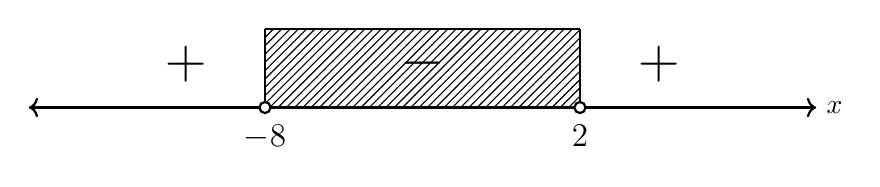
\begin{tikzpicture}

    % Garis bilangan
    \draw[thick,<->] (-5,0) -- (5,0) node[right] {$x$};

    % Arsiran daerah negatif
    \fill[pattern=north east lines] (-2,0) rectangle (2,1);

    % Label titik
    \draw (-2,-0.1) node[below] {\large{$-8$}};
    \draw (2,-0.1) node[below] {\large{$2$}};

    % Tanda batas dan bagian atas
    \draw[thick] (-2,0) -- (-2,1);
    \draw[thick] (2,0) -- (2,1);
    \draw[thick] (-2,1) -- (2,1);

    % Tanda positif-negatif
    \draw (0,0.2) node[above] {\huge{$-$}};
    \draw (3,0.2) node[above] {\huge{$+$}};
    \draw (-3,0.2) node[above] {\huge{$+$}};

    % Titik terbuka
    \draw[fill=white, thick] (-2,0) circle (2pt);
    \draw[fill=white, thick] (2,0) circle (2pt);

\end{tikzpicture}
        \end{center}
        Karena yang diminta adalah nilai \(x\) yang membuat pertidaksamaan \eqref{ineq:soal1} kurang dari nol, maka solusi dari pertidaksamaan tersebut adalah \(-8 < x < 2\). Dalam notasi interval, solusi tersebut dapat ditulis sebagai $\colorlet{oldcolor}{.}
        \color{red}
        \setlength{\fboxrule}{1pt} \boxed{\color{oldcolor}(-8, 2)}\color{oldcolor}$.}
    \end{jawab}
\newpage
    \item Diberikan fungsi \(f(x) = \frac{1}{x-1}\) dan \(g(x) = 2 - \sqrt{x}\).
    \begin{enumerate}
        \item Tentukan domain dari fungsi \(f\) dan \(g\).
        \item Dapatkan fungsi \((f \circ g)(x)\) beserta domainnya.
    \end{enumerate}
    \begin{jawab}[domain fungsi, fungsi komposisi, domain fungsi komposisi]{
        \begin{enumerate}
            \item Diperhatikan bahwa $f(x)$ merupakan fungsi rasional, sehingga domainnya adalah semua bilangan real kecuali nilai yang membuat penyebutnya sama dengan nol. Jadi
            \[
            \colorlet{oldcolor}{.}
        \color{red}
        \setlength{\fboxrule}{1pt} \boxed{\color{oldcolor}D(f)=\{x \in \mathbb{R} : x \neq 1\}}\color{oldcolor}.
            \]
            Selanjutnya, diperhatikan bahwa $g(x)$ memuat akar kuadrat, sehingga domainnya adalah semua bilangan real yang membuat ekspresi di dalam akar kuadrat tak negatif. Jadi 
            \[
            \colorlet{oldcolor}{.}
        \color{red}
        \setlength{\fboxrule}{1pt} \boxed{\color{oldcolor}D(g)=\{x \in \mathbb{R} : x \geq 0\}}\color{oldcolor}.
            \]
            \item Diperhatikan bahwa 
            \begin{align*}
                (f\circ g)(x) = f(g(x)) = f(2 - \sqrt{x}) = \frac{1}{(2 - \sqrt{x}) - 1} = 
                \colorlet{oldcolor}{.}
        \color{red}
        \setlength{\fboxrule}{1pt} \boxed{\color{oldcolor}\frac{1}{1 - \sqrt{x}}}\color{oldcolor}
            \end{align*}
            Domain dari fungsi komposisi $f\circ g$ adalah semua nilai $x$ pada domain $g$ sehingga nilai dari $g(x)$ berada pada domain $f$, yang dapat dirumuskan sebagai 
            \begin{align*}
                \colorlet{oldcolor}{.}
        \color{blue}
        \setlength{\fboxrule}{1pt} \boxed{\color{oldcolor}D(f\circ g) = \{x \in D(g) : g(x) \in D(f)\} = \{x \in [0, \infty) : 2 - \sqrt{x} \neq 1\}}\color{oldcolor}.
            \end{align*}
            Karena $2 - \sqrt{x} = 1$ jika dan hanya jika $\sqrt{x} = 1$, yang berarti $x = 1$, didapatkan
            \begin{align*}
                \colorlet{oldcolor}{.}
        \color{red}
        \setlength{\fboxrule}{1pt} \boxed{\color{oldcolor}D(f\circ g) = [0, \infty) \setminus \{1\} = [0, 1) \cup (1, \infty)}\color{oldcolor}.
            \end{align*}
        \end{enumerate}
    }
        
    \end{jawab}

    \item Diberikan fungsi \(f(x) = \begin{cases} \frac{x^3-8}{2x-4}, & x \neq 2 \\ k, & x=2 \end{cases}\).
    \begin{enumerate}
        \item Tentukan nilai \(k\) sehingga \(f(x)\) kontinu di \(x = 2\).
        \item Berdasarkan hasil dari (a), nyatakan \(f(x)\) sebagai polinomial.
    \end{enumerate}
    \begin{jawab}[fungsi kontinu, limit, polinomial]{
        \begin{enumerate}
            \item Ingat kembali syarat fungsi kontinu di suatu titik \(x = a\) adalah
            \begin{enumerate}
                \item \(f(a)\) terdefinisi
                \item \(\displaystyle \lim_{x \to a} f(x)\) ada, yaitu $\displaystyle \lim_{x \to a^-} f(x) = \lim_{x \to a^+} f(x)$
                \item \(\displaystyle\lim_{x \to a} f(x) = f(a)\)
            \end{enumerate} 
            Diperhatikan bahwa untuk \(x = 2\), \(\colorlet{oldcolor}{.}
        \color{blue}
        \setlength{\fboxrule}{1pt} \boxed{\color{oldcolor}f(2) = k~\text{terdefinisi}}\color{oldcolor}\). Karena limit di $x=2$ artinya nilai fungsi di sekitar $x=2$ tetapi $x\neq 2$, didapatkan limitnya adalah
            \begin{align*}
            \lim_{x \to 2} f(x) = \lim_{x \to 2} \frac{x^3 - 8}{2x - 4} = \lim_{x \to 2} \frac{(x-2)(x^2 + 2x + 4)}{2(x-2)} = \lim_{x \to 2} \frac{x^2 + 2x + 4}{2} = \frac{4 + 4 + 4}{2} = \colorlet{oldcolor}{.}
        \color{blue}
        \setlength{\fboxrule}{1pt} \boxed{\color{oldcolor}6}\color{oldcolor}.
            \end{align*}
            Selanjutnya, untuk syarat ketiga, haruslah $\displaystyle \colorlet{oldcolor}{.}
        \color{blue}
        \setlength{\fboxrule}{1pt} \boxed{\color{oldcolor}\lim_{x \to 2} f(x) = f(2)}\color{oldcolor}$, sehingga diperoleh $\colorlet{oldcolor}{.}
        \color{red}
        \setlength{\fboxrule}{1pt} \boxed{\color{oldcolor}k=6}\color{oldcolor}$.
        \item Diperhatikan bahwa untuk $x\neq 2$, berlaku 
        \begin{align*}
            f(x) = \frac{x^3 - 8}{2x - 4} = \frac{(x-2)(x^2 + 2x + 4)}{2(x-2)} = \frac{x^2 + 2x + 4}{2} = \frac{1}{2}x^2 + x + 2.
        \end{align*}
        Berdasarkan hasil dari (a), diperoleh bahwa \(f(x)\) kontinu di \(x=2\) jika \(k=6\). Dengan demikian, fungsi \(f(x)\) dapat dinyatakan sebagai polinomial
        \begin{align*}
            \colorlet{oldcolor}{.}
        \color{red}
        \setlength{\fboxrule}{1pt} \boxed{\color{oldcolor}f(x) = \frac{1}{2}x^2 + x + 2}\color{oldcolor}.
        \end{align*}
        \end{enumerate}
    }
        
    \end{jawab}

    \item Diberikan fungsi implisit \(3x^2 + y^2 - 2xy + y - x = 6\). Tentukan \(\frac{dy}{dx}\) di titik \((0,-3)\).\\
    \begin{jawab}[diferensiasi implisit, turunan, aturan perkalian, aturan rantai]{~\\
        Diperoleh turunan implisit dari fungsi tersebut dengan menurunkan kedua ruas terhadap \(x\):
        \begin{align*}
            \frac{d}{dx}(3x^2 + y^2 - 2xy + y - x) &= \frac{d}{dx}(6)\\
            \frac{d}{dx}(3x^2) + \frac{d}{dx}(y^2) - \frac{d}{dx}(2xy) + \frac{d}{dx}(y) - \frac{d}{dx}(x) &= 0
        \end{align*}
        Untuk suku-suku yang tidak mengandung \(y\), turunan terhadap \(x\) dapat dihitung langsung. Untuk suku-suku yang mengandung \(y\), digunakan aturan rantai dan aturan perkalian. Misalkan $\colorlet{oldcolor}{.}
        \color{blue}
        \setlength{\fboxrule}{1pt} \boxed{\color{oldcolor}u=y^2}\color{oldcolor}$, maka dengan aturan rantai diperoleh
        \begin{align*}
            \colorlet{oldcolor}{.}
        \color{blue}
        \setlength{\fboxrule}{1pt} \boxed{\color{oldcolor}\frac{du}{dx} = \frac{du}{dy}\frac{dy}{dx} = 2y\frac{dy}{dx}}\color{oldcolor}
        \end{align*}
        Misalkan $\colorlet{oldcolor}{.}
        \color{blue}
        \setlength{\fboxrule}{1pt} \boxed{\color{oldcolor}u=2x}\color{oldcolor}$ dan $\colorlet{oldcolor}{.}
        \color{blue}
        \setlength{\fboxrule}{1pt}\boxed{\color{oldcolor}v=y}\color{oldcolor}$, maka dengan aturan perkalian diperoleh
        \begin{align*}
        \frac{d}{dx}(2xy)=u'v+v'u=y\frac{d}{dx}(2x) + x\frac{dy}{dx}= \colorlet{oldcolor}{.}
        \color{blue}
        \setlength{\fboxrule}{1pt} \boxed{\color{oldcolor}2\left(y + x\frac{dy}{dx}\right)}\color{oldcolor}.
        \end{align*}
        Dengan demikian, diperoleh
        \begin{align*}
            6x + 2y\frac{dy}{dx} - 2\left(y + x\frac{dy}{dx}\right) + \frac{dy}{dx} - 1 &= 0\\
            2y\frac{dy}{dx}  - 2x\frac{dy}{dx} + \frac{dy}{dx}  &= 1+2y-6x\\
            (2y - 2x + 1)\frac{dy}{dx} + (6x - 2y - 1) &= 0\\
            \frac{dy}{dx} &=
            \colorlet{oldcolor}{.}
        \color{red}
        \setlength{\fboxrule}{1pt} \boxed{\color{oldcolor}\frac{1+2y-6x}{(2y - 2x + 1)}}\color{oldcolor}
        \end{align*}
        Selanjutnya, substitusi titik \((0,-3)\) ke dalam persamaan turunan:
        \begin{align*}
            \frac{dy}{dx}\bigg|_{(0,-3)} &= \frac{1+2(-3)-6(0)}{(2(-3) - 2(0) + 1)}= \frac{1-6}{-6 + 1}= \frac{-5}{-5}= \colorlet{oldcolor}{.}
        \color{red}
        \setlength{\fboxrule}{1pt} \boxed{\color{oldcolor}1}\color{oldcolor}.
        \end{align*}
    }
        
    \end{jawab}

    \item Diketahui garis \(g_1: y = -x + 6\) dan garis \(g_2: y = 2x\).
    \begin{enumerate}
        \item Tentukan titik potong kedua garis \(g_1\) dan \(g_2\).
        \item Tentukan titik potong \(g_1\) dengan garis \(x = 1\).
        \item Tentukan pula titik potong \(g_2\) dengan garis \(x = 1\). Gambarkan sketsa ketiga garis \(g_1\), \(g_2\), dan garis \(x = 1\). Hitung luas segitiga yang dibentuk ketiga garis tersebut.
    \end{enumerate}
    \begin{jawab}[persamaan garis,titik potong garis, luas segitiga]{
        \begin{enumerate}
            \item Untuk menentukan titik potong kedua garis, kita samakan persamaan kedua garis, yaitu $-x+6=2x$, sehingga $6=3x$, dan diperoleh $x=2$. Selanjutnya, substitusi \(x = 2\) ke dalam salah satu persamaan garis, misalkan \(g_2\), diperoleh $y=2(2)=4$. Jadi titik potong kedua garis adalah \(\colorlet{oldcolor}{.}
        \color{red}
        \setlength{\fboxrule}{1pt} \boxed{\color{oldcolor}(2,4)}\color{oldcolor}\), misalkan sebagai titik $A$
            \item Untuk menentukan titik potong \(g_1\) dengan garis \(x = 1\), substitusi \(x = 1\) ke dalam persamaan \(g_1\), yaitu $y = -1 + 6 = 5$. Jadi titik potong \(g_1\) dengan garis \(x = 1\) adalah \(\colorlet{oldcolor}{.}
        \color{red}
        \setlength{\fboxrule}{1pt} \boxed{\color{oldcolor}(1,5)}\color{oldcolor}\). Misalkan titik potong tersebut sebagai titik $B$
            \item Untuk menentukan titik potong \(g_2\) dengan garis \(x = 1\), substitusi \(x = 1\) ke dalam persamaan \(g_2\), yaitu $y = 2(1) = 2$. Jadi titik potong \(g_2\) dengan garis \(x = 1\) adalah \(\colorlet{oldcolor}{.}
        \color{red}
        \setlength{\fboxrule}{1pt} \boxed{\color{oldcolor}(1,2)}\color{oldcolor}\). Misalkan titik potong tersebut sebagai titik $C$.\\
            Dengan melakukan plot titik-titik potong tersebut dan menarik garis di antara dua titik potong, didapatkan sketsa dari ketiga garis dan segitiga tersebut adalah sebagai berikut
            \begin{center}
                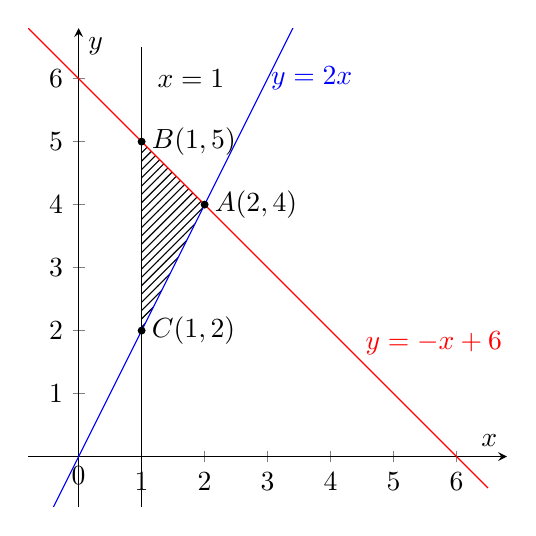
\begin{tikzpicture}
                   \begin{axis}[
x =0.8 cm, y=0.8 cm,
axis lines=middle,
xmin=-0.8,xmax=6.8,
ymin=-0.8,ymax=6.8,
xtick distance=1,
ytick distance=1,
xlabel=$x$,
ylabel=$y$
]
\addplot[opacity=0, domain=1:2, name path=A] {2*x};
\addplot[opacity=0, domain=1:2, name path=B] {-x+6};
% Kurva y = sqrt(x)
\addplot [red,domain=-1:6.5, samples=1000] {-x+6};

% Garis y = 2
\addplot [blue,domain=-1:6.5, samples=1000] {2*x};

% Daerah arsiran
\addplot[pattern=north east lines] fill between[of=A and B, soft clip={domain=1:2}];


% Garis x = 0
\draw (1,-1.5) -- (1,6.5);

% Sumbu putar x = -2
\draw[dashed] (-2,-0.5) -- (-2,3);
\draw (-2.2,2.7) node{$x=-2$};
\draw (1.1,6) node[right]{$x=1$};

% Label kurva
\draw[blue] (3.7,6) node{$y=2x$};
\draw[red] (4.4,1.8) node[right] {$y=-x+6$};
\draw[fill=black, thick] (2,4) circle (1pt) node[right] {$A(2,4)$};
\draw[fill=black, thick] (1,5) circle (1pt) node[right] {$B(1,5)$};
\draw[fill=black, thick] (1,2) circle (1pt) node[right] {$C(1,2)$};
% Label x=0
\draw (0,-0.3) node{$0$};

\end{axis}
                \end{tikzpicture}
            \end{center}
            Pandang garis $BC$ sebagai alas segitiga, sehingga panjang alasnya adalah $|5-2|=\colorlet{oldcolor}{.}
        \color{blue}
        \setlength{\fboxrule}{1pt} \boxed{\color{oldcolor}3}\color{oldcolor}$. Selanjutnya, pandang garis $A$ sebagai titik puncak segitiga, sehingga tinggi segitiga adalah jarak dari titik $A$ ke garis $BC$, yaitu jarak dari titik $(2,4)$ ke garis $x=1$, yang panjangnya adalah $|2-1|=\colorlet{oldcolor}{.}
        \color{blue}
        \setlength{\fboxrule}{1pt} \boxed{\color{oldcolor}1}\color{oldcolor}$. Dengan demikian, luas segitiga tersebut adalah
            \[
            L = \frac{1}{2} \times \text{alas} \times \text{tinggi} = \frac{1}{2} \times 3 \times 1 = \colorlet{oldcolor}{.}
        \color{red}
        \setlength{\fboxrule}{1pt} \boxed{\color{oldcolor}\frac{3}{2}}\color{oldcolor}.
            \]
        \end{enumerate}
    }
    \end{jawab}
\end{enumerate}
\begin{center}
    \large{\textbf{Soal ETS Kalkulus 1 (IUP) ITS Tahun 2025/2026}}
\end{center}
\begin{enumerate}
           \item Solve the following inequality.
    \[ \frac{x^2 - x - 12}{x^2 - 2x - 3} \ge 0 \]

    \item Given a function \(f(x) = 2 - \sqrt{x}\) and \(g(x) = \frac{1}{x-1}\). Determine:
    \begin{enumerate}
        \item[a)] The domain of function \(f\) and \(g\);
        \item[b)] Function \((f \circ g)(x)\) and its domain.
    \end{enumerate}

    \item Write the derivative formula of \(\frac{f}{g}\), that is \(\frac{d}{dx}\left(\frac{f(x)}{g(x)}\right)\). \\
    Then, find the derivative of \(\frac{f}{g}\) given that \(f(x) = 2x^2 + 3x - 2\) and \(g(x) = x - 1\) for \(x \neq 1\).

    \item Given \(f(x) = \begin{cases} \frac{x^3-8}{2x-4}, & x \neq 2 \\ 2k, & x=2 \end{cases}\).
    \begin{enumerate}
        \item[a.] Determine k such that \(f(x)\) continuous at \(x = 2\).
        \item[b.] Based on the result of a), rewrite \(f(x)\) as a polynomial.
    \end{enumerate}

    \item Sketch the base curve \(x = y^2\). Based on that base curve, use translation to sketch the curve \(x = y^2 + 4y + 1\). (Explain the process).

        \end{enumerate}
    


\end{document}


